\documentclass{article}
%\usepackage[latin1]{inputenc}
\usepackage[brazil]{babel}
\usepackage[utf8]{inputenc}
\usepackage[T1]{fontenc}
\usepackage{graphicx}
\usepackage{url}
\newcommand{\R}{{\sf \,R\,}}
\newcommand{\code}[1]{\texttt{#1}}
\title{\normalsize Package sads  \\ Modeling Species Abundance Distributions \\ \large LOGBOOK}
\author{\small Paulo Inácio Prado  and Cristiano Strieder}
 
%\VignetteIndexEntry{Errata corrige to 1st edition of the companion book} 
\usepackage{Sweave}
\begin{document}
\maketitle

\section*{Warning}
Though this document will hopefully become a comprehensive vignette, currently it is a draft logbook used to clarify some aspects of the theoretical background of this package to developers, and to guide the next steps. 

\section*{Poisson Sample}

Given that there is $n$ individuals of a given species in a community and that a fraction $a$ of these individuals were randomly sampled, the probability of getting $y$ individuals in the sample is given by the Poisson distribution

\begin{equation}
  \label{eq:poisson}
f(y)\, = \, \frac{{\left( a\,n\right) }^{y}\,{e}^{-a\,n}}{y!}
\end{equation}

Where the the single parameter of the Poisson $\lambda$ correspond to the expected value $E[y]$ and thus is substituted by the product $a\, n$. Now suppose that the abundance $n$ in the community is also a random variable that can be described by some probability distribution $g(n)$. Then the unconditional probability of getting $y$ individuals in the sample is given by the integral
\begin{equation}
  \label{eq:integral}
  h(y) \, = \, \int^{\Omega}f(y)g(n) \, dn \
\end{equation}

Which is the sad model we are looking for. Although there are analytic solutions for many cases, our goal is to write a  \R  function that solves numerically equation \ref{eq:integral} in a generic way, that is, a single function whith an argument for $g(n)$. This function would then allow to compound any probability density function with the Poisson distribution. Taking this generalization further, we can substitute the Poisson distribution by another sampling model, e.g. the negative binomial to model aggregated sampling.

Our first step is to construct a function for a particular case for which the analytical solution is known, which allow us to check the results of the numerical integration.


\subsection*{Compounding with the exponential}

Taking for $g(n)$ the exponential

\begin{equation}
  \label{equation}
  g(n)\, = \, \lambda\,{e}^{-n\,\lambda}
\end{equation}

The equation \ref{eq:integral} solves to:


\begin{equation}
  \label{eq:poiexp}
  h(y) = \frac{\lambda \, a^y}{(a+\lambda)^{y+1}}
\end{equation}

Using logarithms in the intermediary calculations to avoid overflow, we can define this function in \R as

\begin{Schunk}
\begin{Sinput}
> dpoix <- function(x, frac, rate, log=FALSE) {
+ 	  b <- x*log(frac)
+ 	  m <- log(rate)
+ 	  n <- (x+1)*log(rate+frac)
+           if(log)b+m-n else exp(b+m-n)
+         }
\end{Sinput}
\end{Schunk}


The equivalent function for numerical integration in \R is\footnote{This function must be passed to \code{Vectorize} to make \code{integrate} work with more than one  value of \code{y}}:


\begin{Schunk}
\begin{Sinput}
> dsad <- Vectorize(FUN=
+                   function(y,a,lambda){
+                     poi <- function(y,n){
+                       w <- y*log(a*n)-lfactorial(y)-a*n
+                       exp(w)
+                     }
+                     f1 <- function(n){
+                       dexp(n,rate=lambda) * poi(y,n)
+                     }
+                     integrate(f1,0,Inf, abs.tol = .Machine$double.eps^0.25/1000000)$value
+                   },
+                   "y")
\end{Sinput}
\end{Schunk}

The functions seems to give the same results

\begin{Schunk}
\begin{Sinput}
> dsad(0:10,a=0.1,lambda=0.01)
\end{Sinput}
\begin{Soutput}
 [1] 0.09090909 0.08264463 0.07513148 0.06830135 0.06209213 0.05644739
 [7] 0.05131581 0.04665074 0.04240976 0.03855433 0.03504939
\end{Soutput}
\begin{Sinput}
> dpoix(0:10,frac=0.1,rate=0.01)
\end{Sinput}
\begin{Soutput}
 [1] 0.09090909 0.08264463 0.07513148 0.06830135 0.06209213 0.05644739
 [7] 0.05131581 0.04665074 0.04240976 0.03855433 0.03504939
\end{Soutput}
\end{Schunk}

But as the value of $y$ increases the numeric solution goes to zero. This effect is circumvented by the argument \code{abs.tol}, but it is not yet solved for small values of \code{frac} and \code{rate}, e.g.

\begin{Schunk}
\begin{Sinput}
> dsad(c(200,20000),0.1,0.00001)
\end{Sinput}
\begin{Soutput}
[1] 6.319212e-64 0.000000e+00
\end{Soutput}
\begin{Sinput}
> dpoix(c(200,20000),0.1,0.00001)
\end{Sinput}
\begin{Soutput}
[1] 9.801016e-05 1.353353e-05
\end{Soutput}
\end{Schunk}
The figure \ref{fig:fig01} shows that this effect occurs even for moderate values of $\lambda$. The next step is to investigate this, and to correct the numerical integration.


\begin{figure}[ht]
  \begin{center}
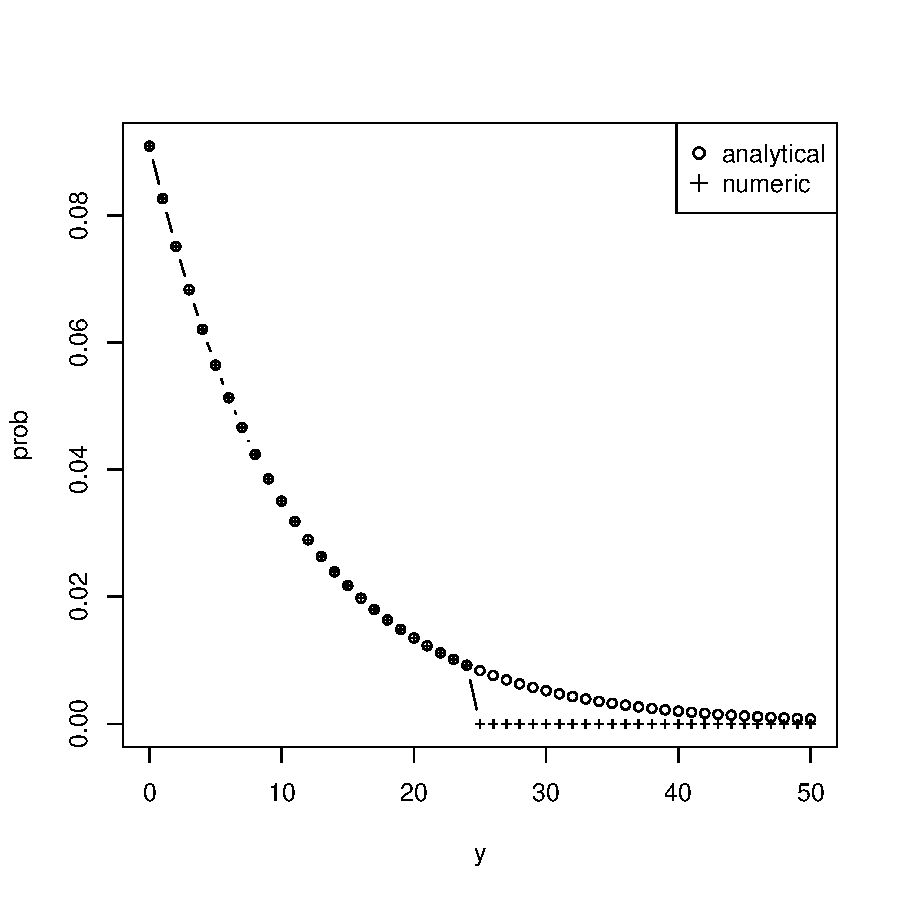
\includegraphics{sads_tutorial-006}
\end{center}
\caption{Probability value returned by the function \code{dpoix}, which calculates the Poisson-exponential analytically and the function \code{dsad}, which calculate the compound distribution by numerical integration.}
\label{fig:fig01}
\end{figure}

\subsection*{Numerical integration with the function \code{integrate}}

The first step on investigating this integration is verify the details of the \code{integrate} function. 
From the R-help of the function, we find that it implements the adaptative quadrature method. Additionally to the 
expression being integrated and the limits of integration, \code{integrate} also allow to specify the absolute(\code{abs.tol}) and relative 
(\code{rel.tol}) accuracy of the function used to approximate the integrand.\footnote{
http://www.amtp.cam.ac.uk/lab/people/sd/lectures/nummeth98/integration.htm}

As was said above, the numeric solution goes to zero as the value of \code{y} increases. And this effect is circumvented specifying a value 
for \code{abs.tol}. Although this approach conduct to a numerical result equivalent to the one otained analytically, it is easily found that for ranges(of the parameter  \code{y} and the values of \code{frac} and \code{rate}) out of the considerated, then the explicit definition of \code{abs.tol} does not help at all. Alternativaly, a similar effect is observated when modifying the upper limit of integration and it is interesting to note that the effects are observated even for wide ranges of the parameters. May be the change on \code{abs.tol} induct a modification in the numerial estimation of \code{Inf}  \footnote{http://en.scientificcommons.org/43526693}.

\subsubsection*{A first guess on replace \code{Inf}}

We now propose another way to circumvent the problem, it consist in manipulate the upper limit of integration \code{Inf}. Such procedure is not recommended according to R-help but for our purposes it seems to produce good results.

With a few trials we found that substitutig \code{Inf} by particular values, this can make the numerical solution matches the anlytical. It is observated that increasing the upper limit, when \code{frac} and \code{rate} are getting lower,  conduct to better aproximation of the numerical integration. Considering $\code{frac}=10^{-1}$ and $\code{rate}=10^{-5}$, with $200 \leq \code{y} \geq 20000$, a reasonably good choice is replace \code{Inf} by \code{k*y/(a+lambda)} with \code{k=1.9920941}. Figure \ref{fig:k} shows the analytical and numerical curves visually matching. Figure \ref{fig:abs.tol} is the result when integral is calculated with \code{abs.tol}.

\begin{figure}[ht]
  \begin{center}
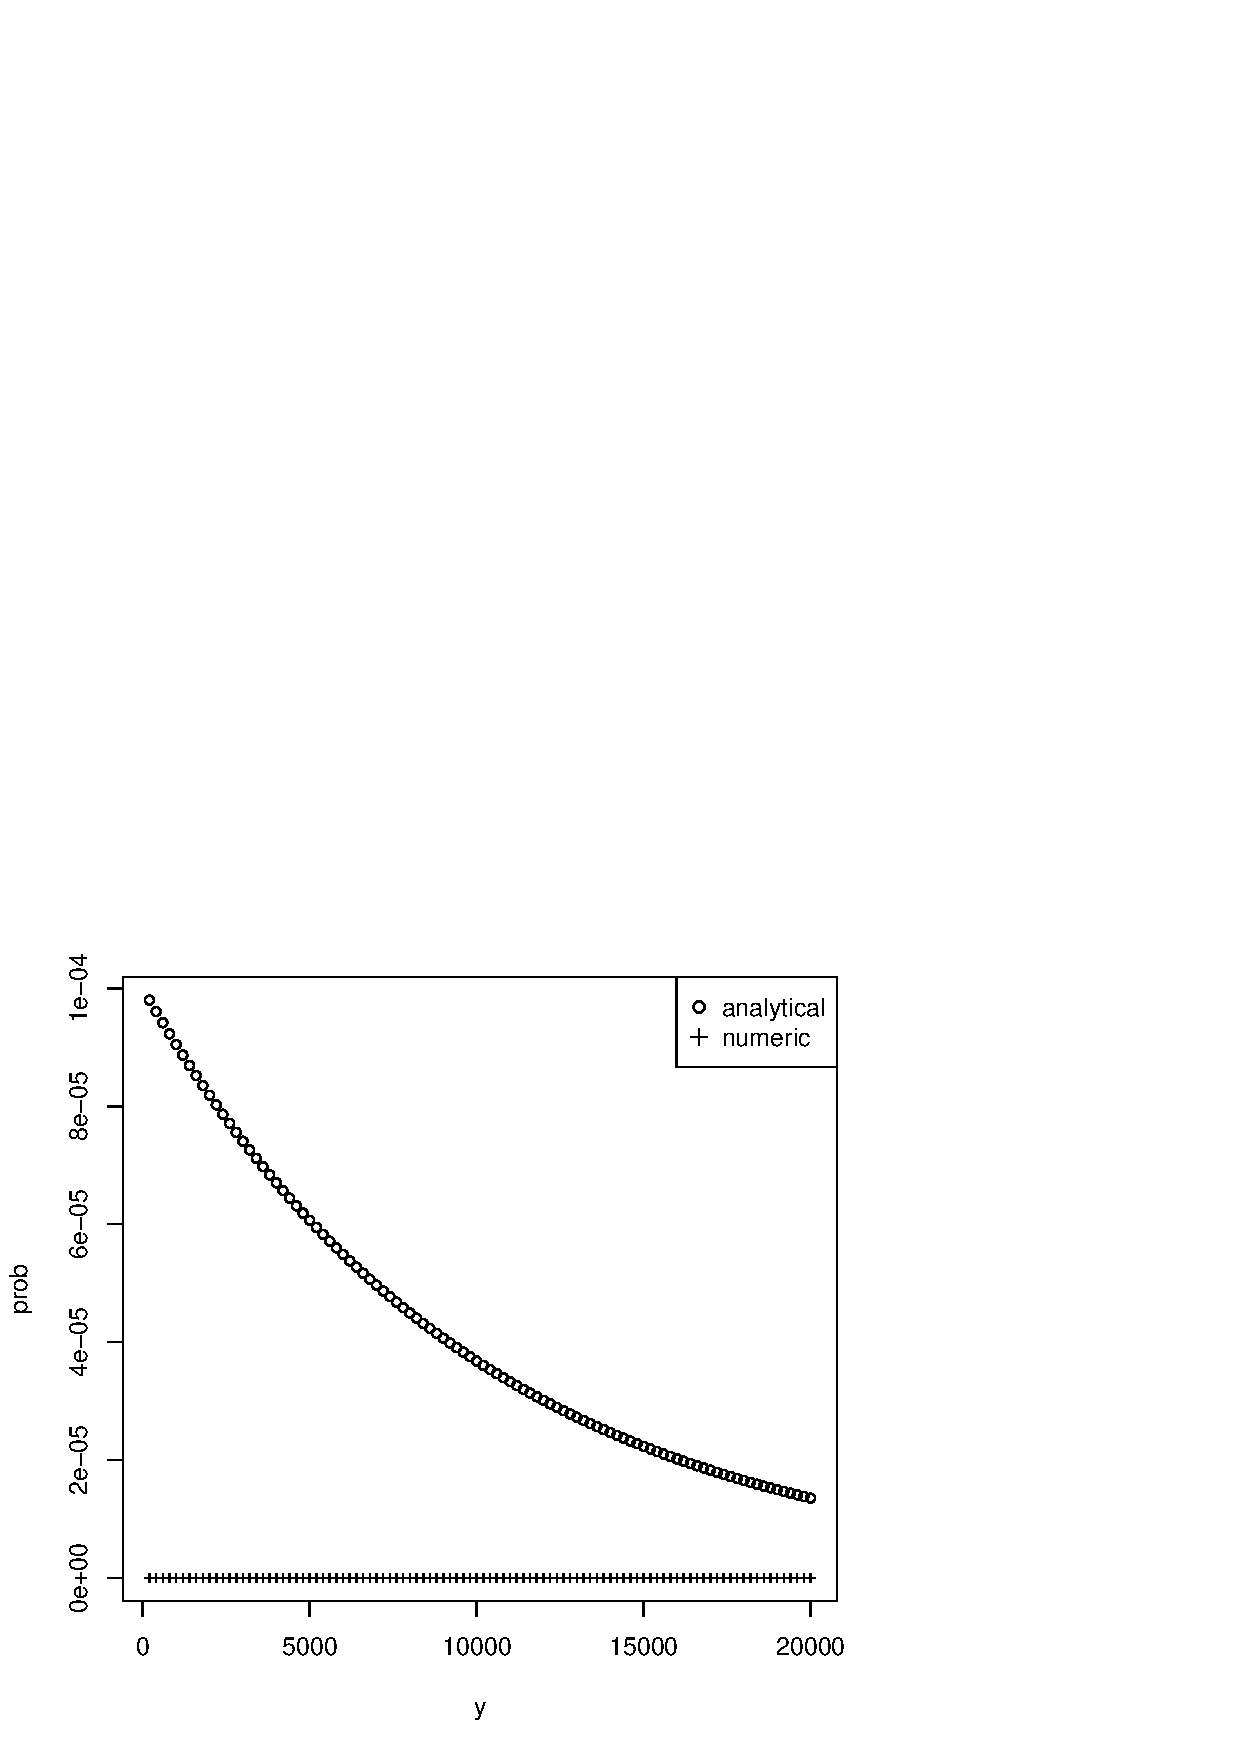
\includegraphics{sads_tutorial-007}
\end{center}
\caption{Probability value returned by the function \code{dpoix} and the function \code{dsad}. Considering $\code{frac}=10^{-1}$ and $\code{rate}=10^{-5}$, with $200 \leq \code{y} \geq 20000$}.
\label{fig:abs.tol}
\end{figure}

y1 <- dpoix(x,frac,rate)

\begin{figure}[ht]
  \begin{center}
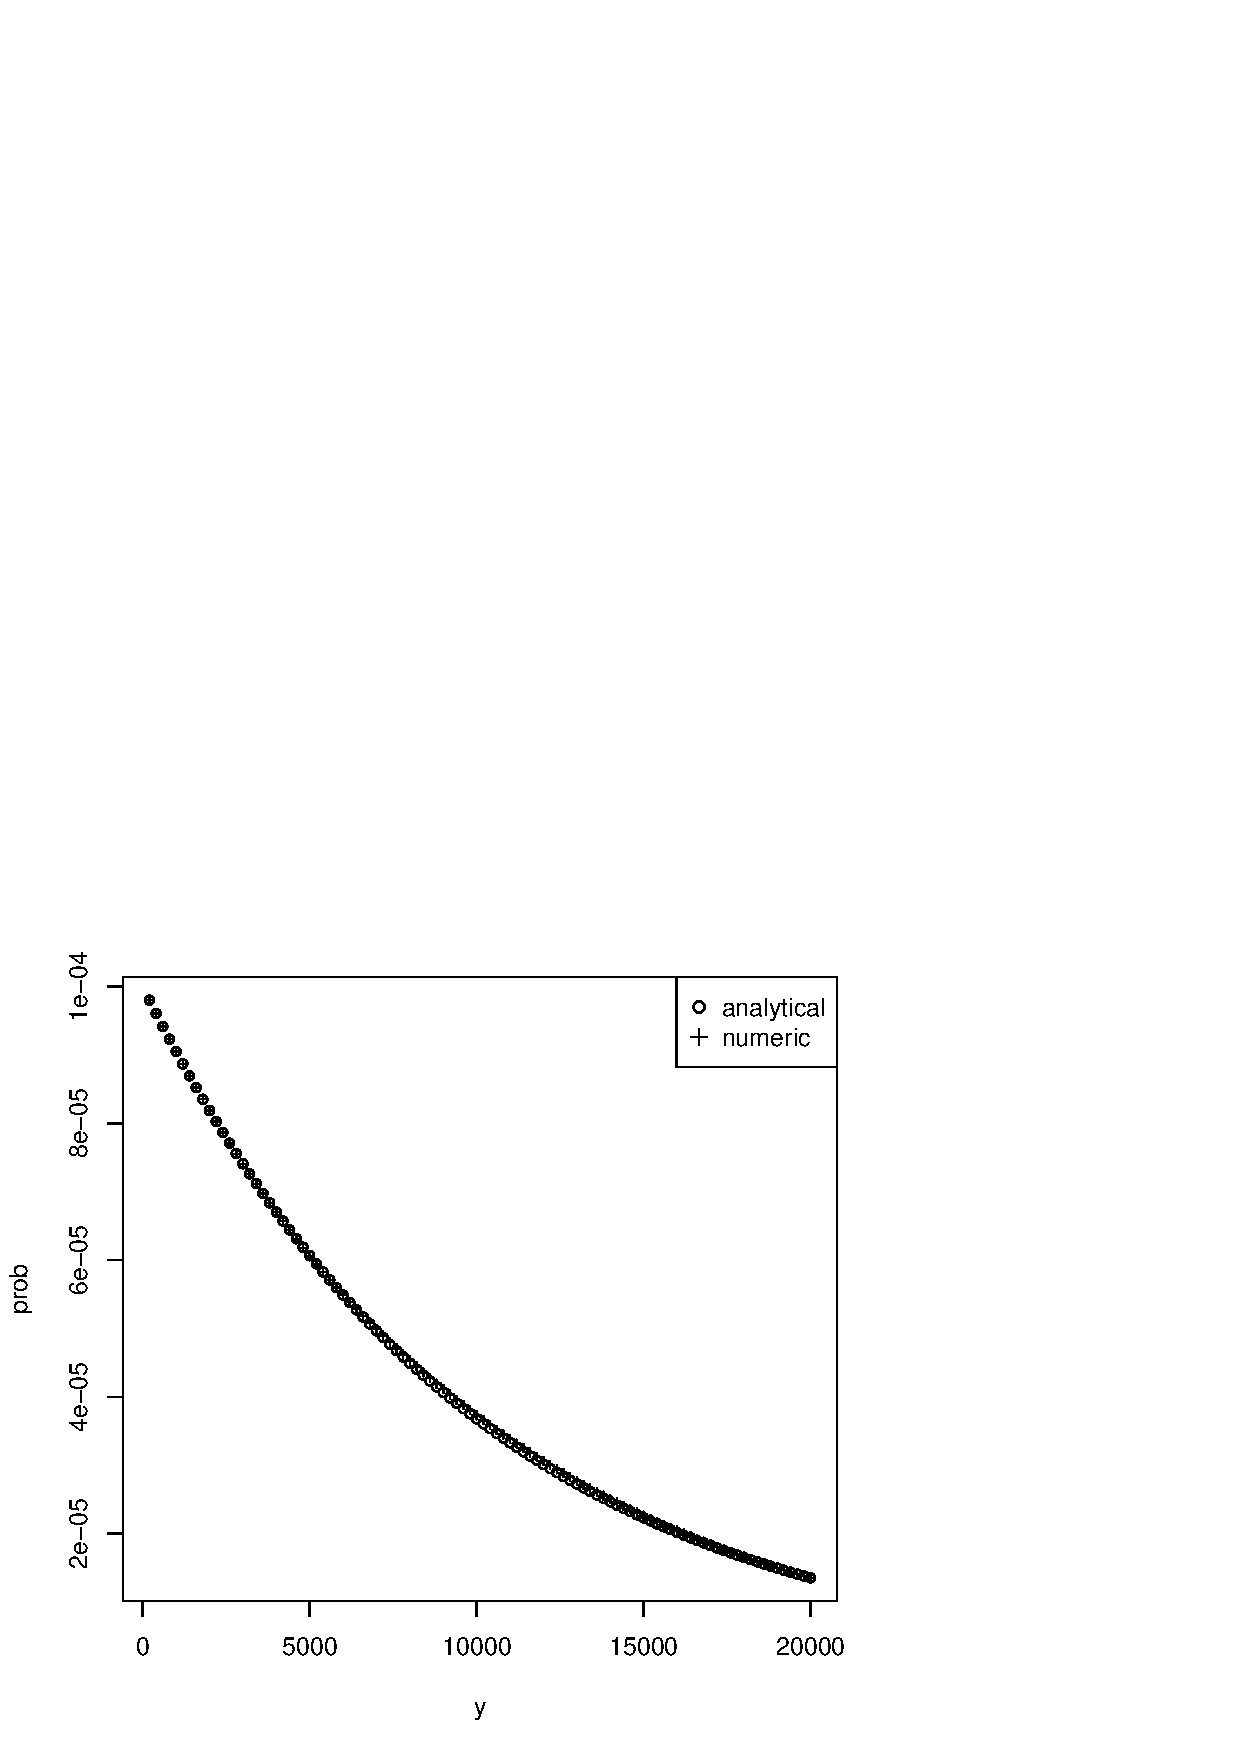
\includegraphics{sads_tutorial-009}
\end{center}
\caption{Probability value returned by the function \code{dpoix} and the function \code{dsad}. Considering $\code{frac}=10^{-1}$ and $\code{rate}=10^{-5}$, with $200 \leq \code{y} \geq 20000$}
\label{fig:k}
\end{figure}

In the above case the value of \code{k} was manually tunned, hopefully giving exact results for:

\begin{Schunk}
\begin{Sinput}
> dsad(c(200,20000),0.1,0.00001)
\end{Sinput}
\begin{Soutput}
[1] 9.801016e-05 1.353353e-05
\end{Soutput}
\begin{Sinput}
> dpoix(c(200,20000),0.1,0.00001)
\end{Sinput}
\begin{Soutput}
[1] 9.801016e-05 1.353353e-05
\end{Soutput}
\end{Schunk}

For ranges out of the cited above, then the value of \code{k}, or even the entire solution, may be defined more consistently. This result can be improved, for wide ranges of \code{frac}, \code{rate} and \code{y}, if we specify 
the upper limit of integration in an another alternative manner. This time the idea is to split the total range of any parameter, \code{y} for example, in two or more parts and then specify the numerical integration for each part, as is shown below.

\begin{Schunk}
\begin{Sinput}
> dsad <- Vectorize(FUN=
+                   function(y,a,lambda){
+                     poi <- function(y,n){
+                       w <- y*log(a*n)-lfactorial(y)-a*n
+                       exp(w)
+                     }
+                     f1 <- function(n){
+                       dexp(n,rate=lambda) * poi(y,n)
+                     }
+ 					if (y<10){
+ 						integrate(f1,0,100/max(a,lambda))$value
+ 					}else if (y<50){
+ 						k <- 6
+ 						integrate(f1,0,k*y/(a+lambda))$value
+ 					}else{
+ 						k <- 1.9920941
+ 						integrate(f1,0,k*y/(a+lambda))$value
+ 					}
+                   },
+                   "y")
\end{Sinput}
\end{Schunk}

The above expression is an attempt to correct the result from the numerical  integration provided by the standart \code{integrate} R function. The limits for each \code{y} interval were selected to exemplify.

In fact, this is not a final solution yet, but results are improved as shows Figure  \ref{fig:good}. Unfortunately both curves do not match for all ranges. Figure \ref{fig:bad} show an example when it does not work, for $\code{rate}=10^{-6}$\ and\ $\code{frac}=10^{-1}$. Another methods/functions for numerical integration must be tested.

\begin{figure}[ht]
  \begin{center}
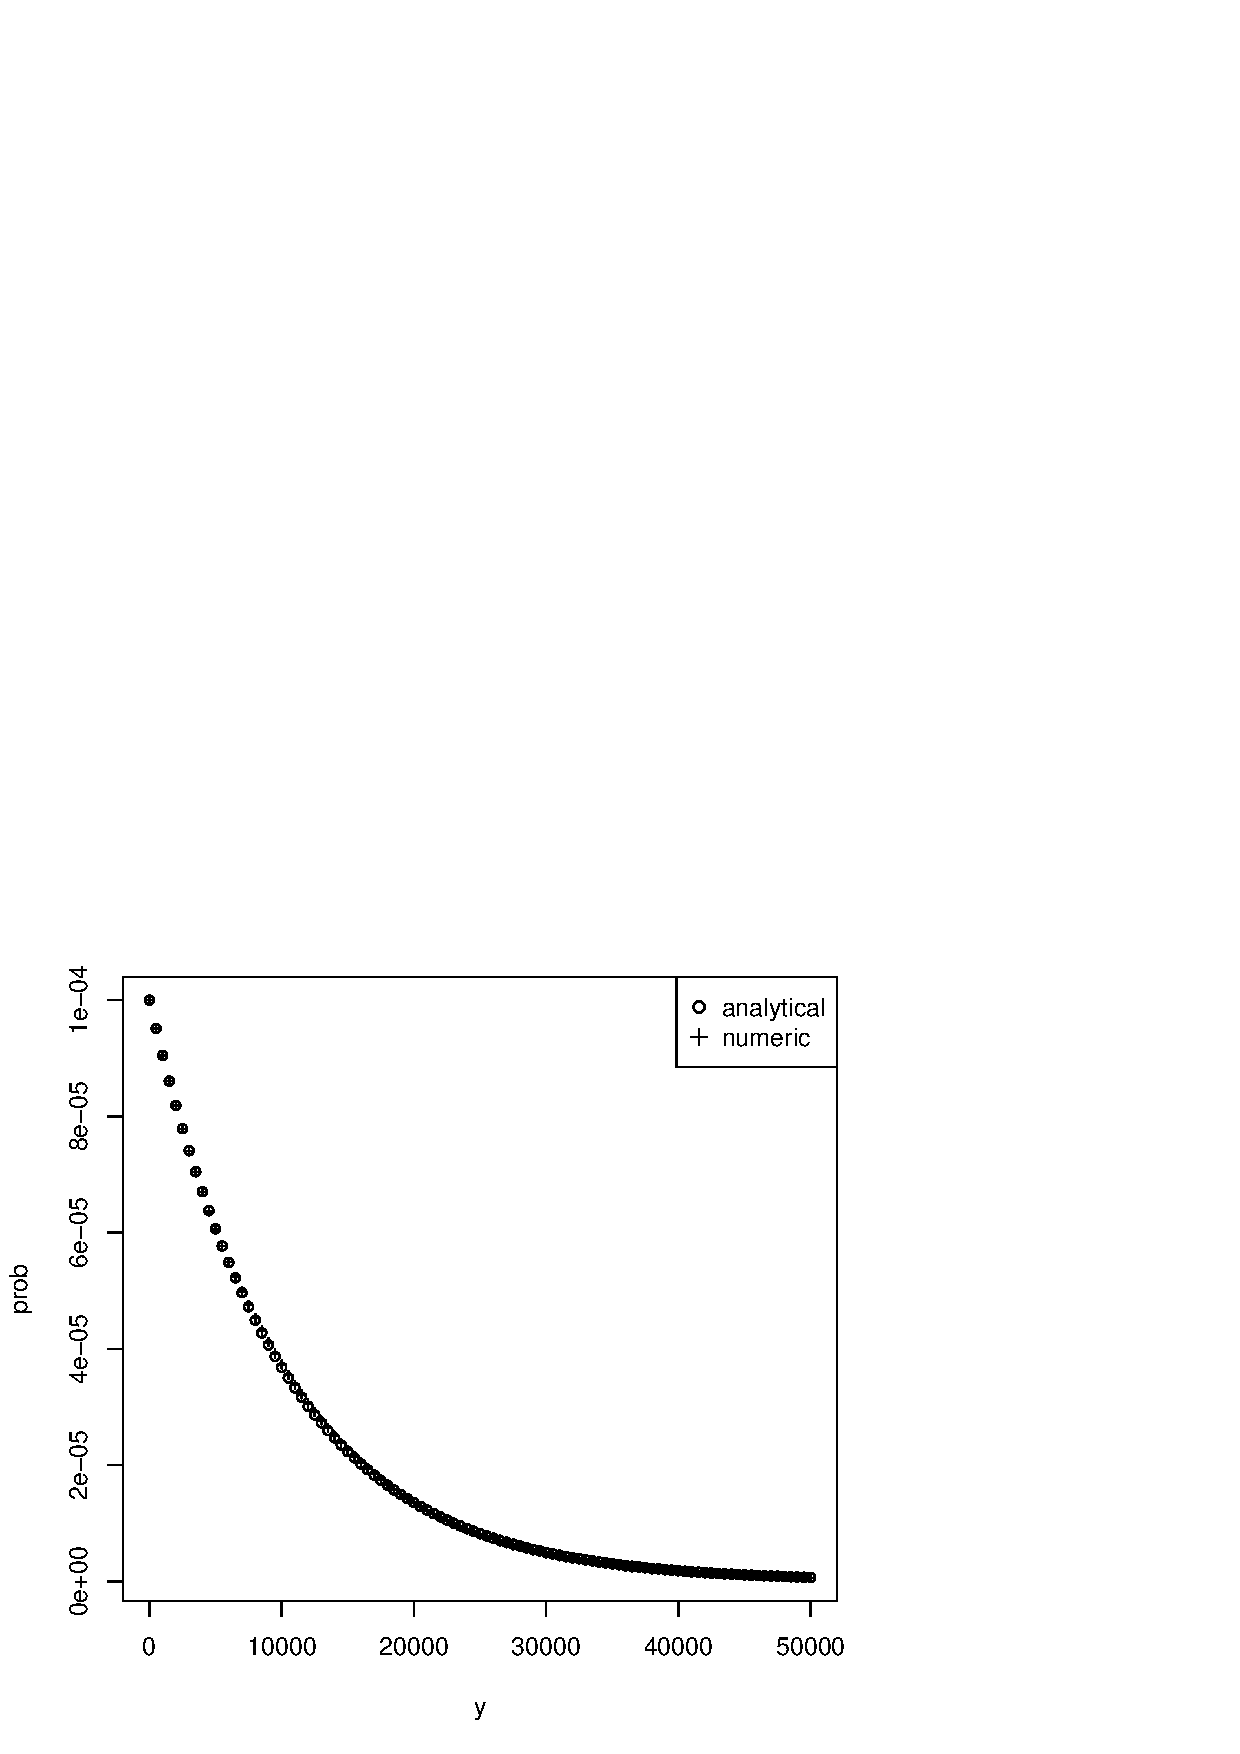
\includegraphics{sads_tutorial-012}
\end{center}
\caption{Probability value returned by the function \code{dpoix} and the function \code{dsad}. Considering $\code{frac}=10^{-1}$ and $\code{rate}=10^{-5}$, with $0 \leq \code{y} \geq 50000$}
\label{fig:good}
\end{figure}

\begin{figure}[ht]
  \begin{center}
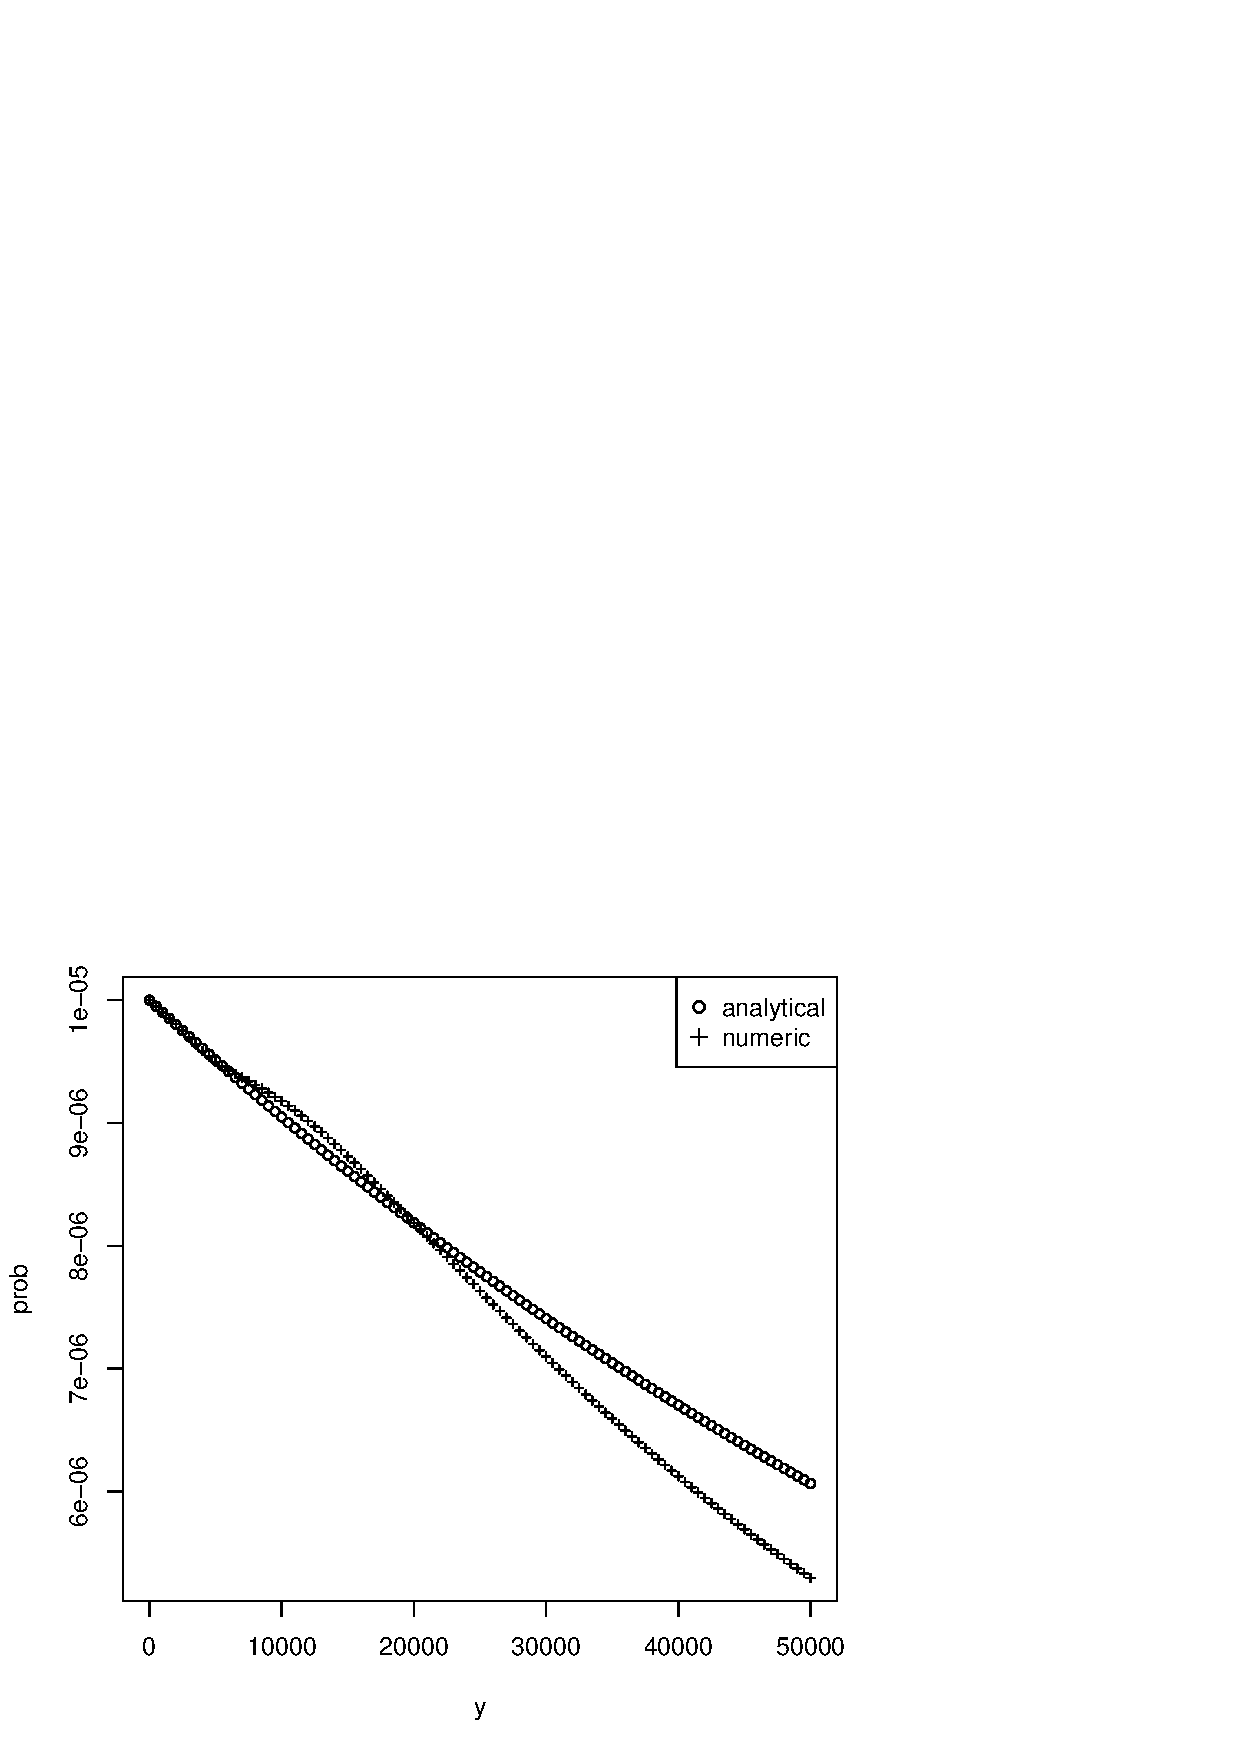
\includegraphics{sads_tutorial-013}
\end{center}
\caption{Probability value returned by the function \code{dpoix} and the function \code{dsad}. Considering $\code{frac}=10^{-1}$ and $\code{rate}=10^{-6}$, with $0 \leq \code{y} \geq 50000$}
\label{fig:bad}
\end{figure}

\subsubsection*{A general criteria to set the upper integration limit}
An abundance value that is larger than the abundances of all or most of the  species in the community is a natural upper limit for the integration. This value can be set with the quantile functions of the probability distibutions. For example, for a community sad that follow a gamma distribution with parameters \code{rate=0.000075} and \code{shape=0.75} \footnote{These are the values used by Green \& Plotkin fig. 1}, 99.99\% of the species will have an abundance below:

\begin{Schunk}
\begin{Sinput}
> qgamma(0.9999,rate=0.000075, shape=0.75)
\end{Sinput}
\begin{Soutput}
[1] 112629.0
\end{Soutput}
\end{Schunk}

This provides an abundance high enough to be used as upper integration limit, and that can be used with any community sad distribution, since all density functions has the \code[q] quantile function. Initial tests suggest that this may provide a general solution (see below in the section on generalization of the function), but systematic evaluation with a wide range of values is still to be done.

\subsection*{Numerical Integration with function \code{GLIntegrate}}

Package \code{distr} provide an object oriented implementation of distributions. Additionaly, package \code{distrEx} provide extensions of package distr. That extensions include two functions for integration: \code{GLIntegrate} and \code{distrExIntegrate}.

The R-help description of the \code{GLIntegrate} function says it use Gauss-Legendre quadrature over a finite interval, in contrast with our problem that has an infinite upper limit. 

The \code{distrExIntegrate} function does not have the same limitation relative to the interval of integration. But, as the description of the function explain, it does a numerical integration via \code{integrate}, in case \code{integrate} fails a Gauss-Legendre quadrature is performed.

Figures \ref{fig:GLIntegrate} and \ref{fig:distrExIntegrate} shows the result from using \code{GLIntegrate} and \code{distrExIntegrate} respectively. As expected, from the description of the function, \code{distrExIntegrate} exibits a shape like the one got from \code{integrate}.


\begin{figure}[ht]
  \begin{center}
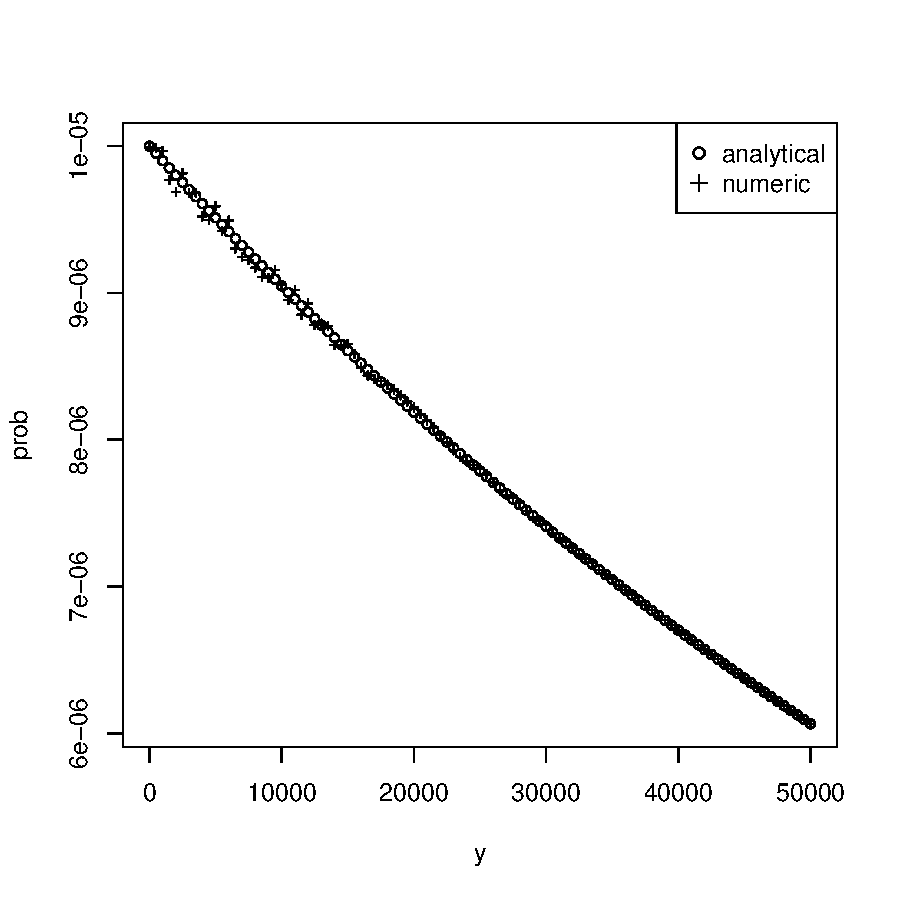
\includegraphics{sads_tutorial-016}
\end{center}
\caption{Probability value returned by the function \code{dpoix} and the function \code{dsad}. Considering $\code{frac}=10^{-1}$ and $\code{rate}=10^{-6}$, with $0 \leq \code{y} \geq 50000$. For the upper limit of integration it was used $10^{6}$.}
\label{fig:GLIntegrate} For the 
\end{figure}



\begin{figure}[ht]
  \begin{center}
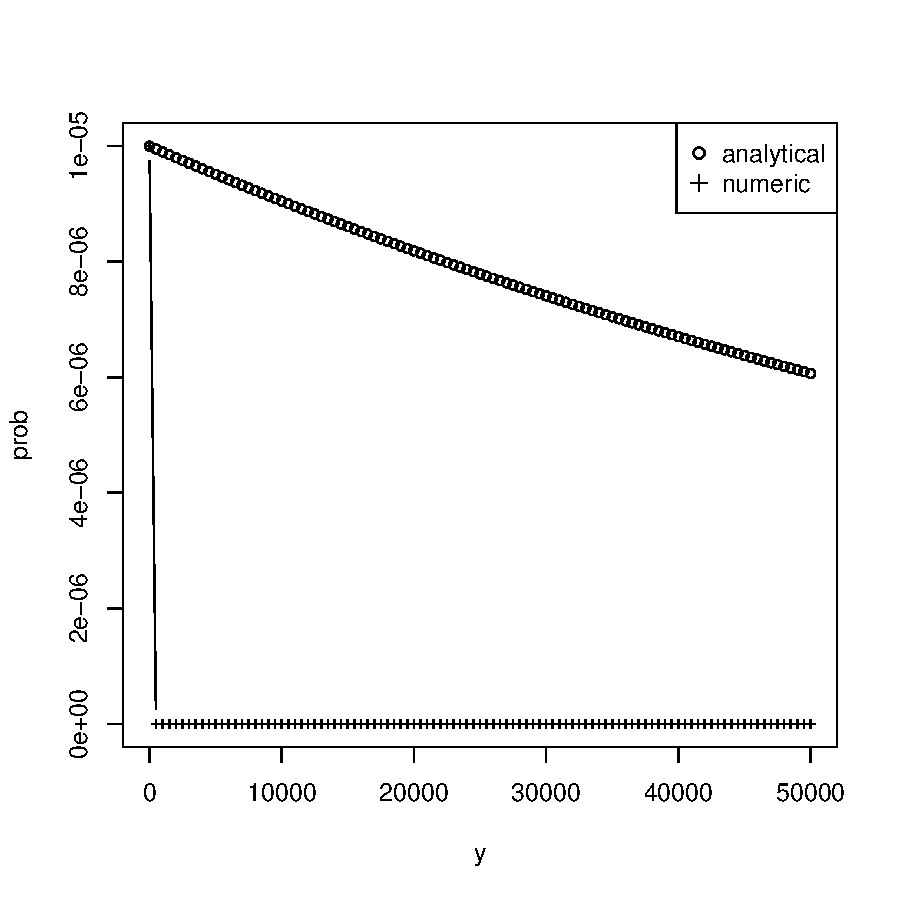
\includegraphics{sads_tutorial-018}
\end{center}
\caption{Probability value returned by the function \code{dpoix} and the function \code{dsad}. Considering $\code{frac}=10^{-1}$ and $\code{rate}=10^{-6}$, with $0 \leq \code{y} \geq 50000$. For the upper limit of integration it was used \code{Inf}.}
\label{fig:distrExIntegrate}
\end{figure}


\subsection*{Numerical Integration with function \code{adaptIntegrate}}

The function \code{adaptIntegrate} come with the Cubature package. Cubature is a package for mutidimensional integration over hypercubes.

Installation can be performed with:


\begin{Schunk}
\begin{Sinput}
> library("cubature")
> dsad <- Vectorize(FUN=
+                   function(y,a,lambda){
+                     poi <- function(y,n){
+                       w <- y*log(a*n)-lfactorial(y)-a*n
+                       exp(w)
+                     }
+                     f1 <- function(n){
+                       dexp(n,rate=lambda) * poi(y,n)
+                     }
+   				 adaptIntegrate(f1,0,10^6)$integral
+                   },
+                   "y")
\end{Sinput}
\end{Schunk}
\begin{figure}[ht]
  \begin{center}
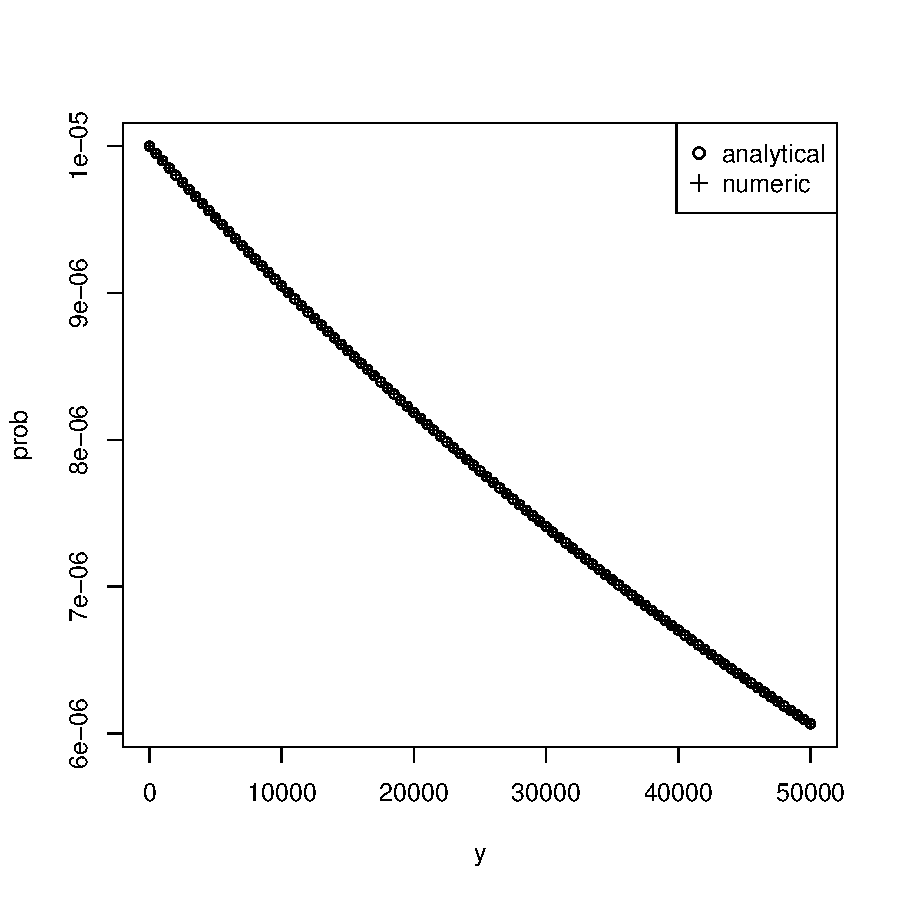
\includegraphics{sads_tutorial-021}
\end{center}
\caption{Cubature. Probability value returned by the function \code{dpoix} and the function \code{dsad}. Considering $\code{frac}=10^{-1}$ and $\code{rate}=10^{-6}$, with $0 \leq \code{y} \geq 50000$}
\label{fig:bad}
\end{figure}


\subsection*{Some aspects of the numerical integration}

One important aspect to verify when dealing with Probability Density Functions - PDFs, is that the sum of probabilities over the entire length is 1. This is tested for both \code{dpoix} and \code{dsad} with the \code{R} function \code{sum}.

%<<tests4>>=
%x <- 0:j
%y1 <- dpoix(x,frac,rate)
%y2 <- dsad(x,frac,rate)
%sum(y1)
%sum(y2)
%@


\subsection*{Compounding with the gamma}

 
Taking for $g(n)$ the gamma

\begin{equation}
\label{eq:gamma}
  g(n) = \frac{ \lambda^{\beta} n^{\beta-1} e^{- \lambda n} }{ \Gamma(\beta) }
\end{equation}

The equation \ref{eq:integral} solves to:

\begin{equation}
  \label{eq:poig}
  h(y) = \frac{a^y \lambda^\beta \Gamma(y+\beta)}{y!\Gamma(\beta)(a+\lambda)^{y+\beta}}
\end{equation}

We can define this function in \R as

\begin{Schunk}
\begin{Sinput}
> dpoig <- function(x, frac, rate, shape) {  
+   b <- (frac^x)*(rate^shape)*gamma(x+shape)
+   c <- factorial(x)*gamma(shape)*(frac+rate)^(x+shape)
+   b/c
+ }
\end{Sinput}
\end{Schunk}

The equivalent function for numerical integration in \R is:

\begin{Schunk}
\begin{Sinput}
> dsad_gamma <- Vectorize(FUN=
+ function(y,a,lambda,shape=0.75,fn=2){
+   poi <- function(y,n){
+     w <- y*log(a*n)-lfactorial(y)-a*n
+     exp(w)
+   }
+   if(fn==1){
+     f1 <- function(n){
+       dexp(n,rate=lambda) * poi(y,n)
+     }
+   }else{  				
+     f1 <- function(n){
+       dgamma(n, shape, rate = lambda, scale = 1/rate) * poi(y,n)
+     }
+   }
+   if (y<10){
+   	integrate(f1,0,100/max(a,lambda))$value
+   }else if (y<50){
+   	k <- 6
+   	integrate(f1,0,k*y/(a+lambda))$value
+   }else{
+   	k <- 1.9920941
+   	integrate(f1,0,k*y/(a+lambda))$value
+   }
+ },
+ "y")
\end{Sinput}
\end{Schunk}

The functions seems to give the same results

\begin{Schunk}
\begin{Sinput}
> frac <- 10^-1
> rate <- 10^-1
> x <- c(1, 10, 50, 100)
> shape <- 0.75
> dsad_gamma(x,frac,rate,shape,fn=2)
\end{Sinput}
\begin{Soutput}
[1] 2.229763e-01 2.640021e-04 1.617665e-16 1.209309e-31
\end{Soutput}
\begin{Sinput}
> dpoig(x,frac,rate,shape)
\end{Sinput}
\begin{Soutput}
[1] 2.229763e-01 2.640021e-04 1.617665e-16 1.209309e-31
\end{Soutput}
\end{Schunk}

\subsection*{General Function}
The purpose is to generalize the function to allow the combination of Poisson or Binomial Negative sampling with any distribution in the community. The current version of this generalized function includes the upper limit set by the quantile criteria, and some tweaks to avoid some of the biases related above:

\begin{Schunk}
\begin{Sinput}
> dsad <- function(y,frac,sad,samp="Poisson",log=FALSE,upper=0.9999,...){
+   qcom <- paste("q",deparse(substitute(sad)),sep="")
+   dcom <- paste("d",deparse(substitute(sad)),sep="")
+   dots <- c(as.name("n"),list(...))
+   uplim <- do.call(qcom,c(upper,list(...)))
+   f1 <- function(z){
+     f2 <- function(n){
+       t1 <- do.call(dcom,dots)
+       t2 <- dpois(z,frac*n)
+       ifelse(t1==0|t2==0,0,t1*t2*1e12)
+     }
+   integrate(f2,0,uplim,rel.tol=sqrt(.Machine$double.eps),subdivisions=500)$value
+   }
+   res <- sapply(y,f1)/(1e12*upper)
+   if(log)log(res) else res
+ }
\end{Sinput}
\end{Schunk}

Some observations:

\begin{itemize}
\item First working version substituted the old version of \code{dsad}
\item A first version of the help page is already done, see for details
\item The function no uses \code{dpois} for the Poisson distribution
\item \code{rel.tol} and \code{subdivisions} increased following \url{https://stat.ethz.ch/pipermail/r-help/attachments/20100921/56db7df0/attachment.pl}
\item \code{log} argument added; necessary to model fitting by maximum likelihood
\item arguments to be passed to the community distribution choosen by \code{sad} vary, and are all under \code{...}. They should be named.
\item Old functions removed from the directory
\end{itemize}
\section*{To Do List}

\begin{enumerate}
\item Functions with analytical solution for Poisson-truncated hyperbolic
\item To use \code{dnbinom} to check \code{dpoig}: a compound Poisson-gamma is a negative binomial for integers, so they must give the same results. 
\item To set the parameters of \code{dpoig} to match the parameters of \code{dnbinom}
\item To standardize arguments and their names across the density functions. 
\item To check the thoroughly compound solutions of the generic function \code{dsads} against their analytical counterparts (\code{dpoix}, \code{dpoig} \ldots)  
\item After all checks with Poisson sampling were done and OK, proceed to set the functions for Binomial Sampling (Table 2 of Green \& Plotkin).
\end{enumerate}

\end{document}
